\documentclass{article}
\usepackage[margin=1in]{geometry}
\usepackage{graphicx}
\usepackage{subcaption}
\usepackage{float}
\renewcommand{\familydefault}{\sfdefault}
\title{Introduction to Pattern Recognition Homework 1}
\author{Andres Ponce(0616110)}
\begin{document}
\maketitle

\section{Program Report} %%tentative section name

		\subsection{Plot the learning curve of the training, you should 
				find that loss decreases after a few iterations 
				(x-axis=iteration,y-axis=loss, Matplotlibor other plot tools is available to use)}

				For this assignment, we plotted both the actual regression function and the error
				for each iteraiton of the training and test data sets. For the original testing, 
				the number of iterations was 100, however, after about 200 iterations, the error
				does not decrease as much. \texttt{main.py} by default runs 1000 iterations for a 
				more accurate result.

				%the !ht places the figures in the actual place in the file
				\begin{figure}[!ht]
					\centering
						\begin{subfigure}{0.4\linewidth}
						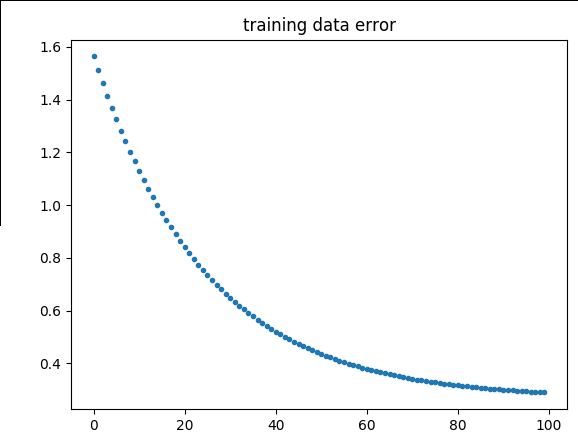
\includegraphics[width=\linewidth]{training_data_error.png}
					\end{subfigure}
					\begin{subfigure}{0.4\linewidth}
						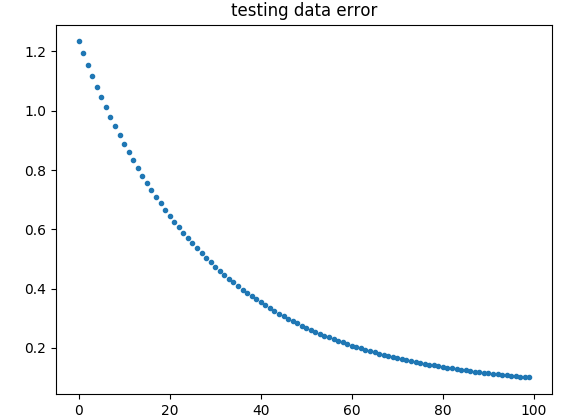
\includegraphics[width=\linewidth]{testing_data_error.png}
					\end{subfigure}
				\end{figure}

		\subsection{What's the Mean Square Error of your prediction and ground truth
				(prediction=model(x\_test),ground truth = y\_test)}

				The error for the testing data  is around 0.26, an around 0.06 for 
				the testing data.
		\subsection{What're the weights and intercepts of your linear model?}

				For the testing data, we got about 0.817 for our slope and 0.784 for our 
				y-intercept.

		\subsection{What's the difference between the Gradient Descent, Mini-Batch Gradient
				Descent, and Stochastic Gradient Descent?}
				
				Gradient Descent seeks to find the minimum to a function. To do this, at each 
				iteration we have to find the \textbf{gradient}, or the how much the slope changes
				at that point. Once we do that, we move in the direction of the gradient (we 
				\textit{descend} along the line), by a factor that depends on the learning rate.
				Eventually, depending on the number of iterations, we should reach a point 
				on or around the global minimum.

				Depending on the amount of data available, it might be infeasible to calculate
				the gradient in a straightforward manner. In \textbf{stochastic gradient descent},
				we pick a random sample from the data points and calculate the gradient based on that
				sample. When the input data is too large to use the entire data set every iteration,
				a stochastic approach might greatly reduce the computational complexity. However,
				the amount of iterations required to achieve the same results also increases. In the end,
				for some applications in big data, this tradeoff might be worth it.

				There exists another approach to the gradient, used in \textbf{mini-batch gradient descent}.
				Here, we only consider a small portion of the training set in  order to make a calculation
				on how to proceed. Since stochastic gradient descent might update the parameters in a noisy 
				manner, mini-batch might present a better alternative for the gradient computation.

				In the end however, all three methods have the goal of minimizing the function to find the 
				correct parameters, with compromises of speed and accuracy.


\section{Questions}


		\subsection{Suppose that we have three colored boxes $R$ (red), $B$ (blue),
				and $G$ (green). Box $R$ contains 3 apples, 4 oranges, and 3 guavas,
				box $B$ contains 2 apples, 0 oranges, and 2 guavas, and box $G$ contains
				12 apples, 4 oranges, and 4 guavas. If a box is chosen at random with 
				probabilities $p(R)=0.2,p(B)=0.4,p(G)=.4$, and a piece of fruit is removed
				from the box (with equal probability of selecting any of the items in the box),
				then what is the probability of selecting guava? If we observe that the selected
				fruit is in fact an apple, what is the probability that it came from the blue box?}

		For the first question, let $b_{i}$ refer to choosing box $i$, and $g_{i}$ refer 
		to choosing a guava from box $i$. If we want the probabilites in general of choosing
		a guava from each of the boxes, we need to add the products $p(b_{i})p(g_{i})$. Thus 
		our formula becomes 
				\[ \sum_{i=0}^{N}p(b_{i})p(g_{i})\]
		which evaluates to 
				\[(.3)(.2) + (.5)(.4) + (.4)(.2) = 0.34\]
		
		For the second question, we want to calculate the probability that the blue box was chosen
		given that we have chosen an apple. Let $a$ be the event of choosing an apple, and $B$ be
		the event of choosing the blue box. Then, we would like to find $p(B|a)$. By using
		\textbf{Baye's Theorem}, which states
		\[ p(A|B) = \frac{p(B|A)p(A)}{p(B)}\]
		we can find each of the required probabilities. We are given that $p(B) = .4$. To find
		$p(a|B)$, we find the probability of choosing an apple from box $B$, which is 
		$\frac{2}{2+2} = 0.5$. Finally, to find $p(a)$, we repeat the process from the first part,
		and add the probabilities of choosing box $i$ and picking an apple from that box, which in the
		end comes out to .5. Thus, our final calculation is 
				\[ p(B|a) = \frac{(.5)(.4)}{(.5)} = .4\]


		\subsection{Using the definition \[\textrm{var}[f] = E[(f(x) - E[f(x)])^{2}] \]
		 show that $\textrm{var}[f(x)]$ satisfies
		\[\textrm{var}[f(x)] = E[f(x)^{2}] - E[f(x)]^{2}\]}
		
		First, we take the first definition of variance and expand the square.
		\[ E[(f(x) - E[f(x)])^{2}] = E[f(x)^{2}] - f(x)E[f(x)] - (E[f(x)])(f(x) - E[f(x)])\]
		For the first two terms, we get
		%\[ \]
		\begin{equation}
				E[f(x)^{2}] - E[f(x)]E[f(x)]
			\label{eq:1}
		\end{equation}
		which becomes
		\begin{equation}
			\label{eq:2}
			 E[f(x)^{2}] - E[f(x)]E[f(x)]
		\end{equation}
		\begin{equation}
				\label{eq:3}
			 = E[f(x^{2})] - E[f(x)]^{2}
		\end{equation}

		because $E[E[f(x)]]$ is simply $E[f(x)]$ because it is a constant term. Therefore we distribute the outer
		$E[]$ to arrive at Equation \ref{eq:3}.

		However, we still have the last copule terms. But,
		\[ E[(E[f(x)])(f(x) - E[f(x)])]\]
		\[ = (E[(f(x)])E[f(x) - E[f(x)]]\]
		\[ = (E[f(x)])(E[f(x)] - E[f(x)]) = 0\]
		So, in the end we are left with Equation \ref{eq:1}, which simplifies to $E[f(x)^{2}] - E[f(x)]^{2}$.
\end{document}
